%\section{Adiabatic approximation}
%\label{sec:dis}
%\subsection{Adiabatic invariant}
For the resonant electrons trapped by the slowly varying wave envelope and circling around in the phase space,  the adiabatic invariant is defined as
\begin{equation}\label{eq.def_I}
    \mathcal{I} = \frac{1}{2\pi} \oint \Omega(H,\xi,t) \mathrm{d} \xi~.
\end{equation}
The integration is over a complete cycle of the coordinate $\xi$.
Here the canonical momentum $\Omega$ is expressed as an implicit function of the Hamiltonian $H$.
Using the Hamiltonian (\ref{eq.H_lab}) and (\ref{eq.H_frame}), 
we can numerically calculate the adiabatic invariant $\mathcal{I}$  in the static and moving resonance frames, respectively.
For each temporospatial location, with fixed background and wave parameters, we are able to complete a closed trajectory if the particle stay trapped in the wave field.  
The area of the enclosed loop is actually the phase space integral $\mathcal{I}$.
In the static frame, it is clear that the area changes significantly,
as shown in Fig. \ref{fig.traj}(c). In the moving frame, the area changes much smaller, suggesting the validity of the particle adiabatic motion, as shown in Fig. \ref{fig.traj}(d). 



\begin{figure}
    \centering
    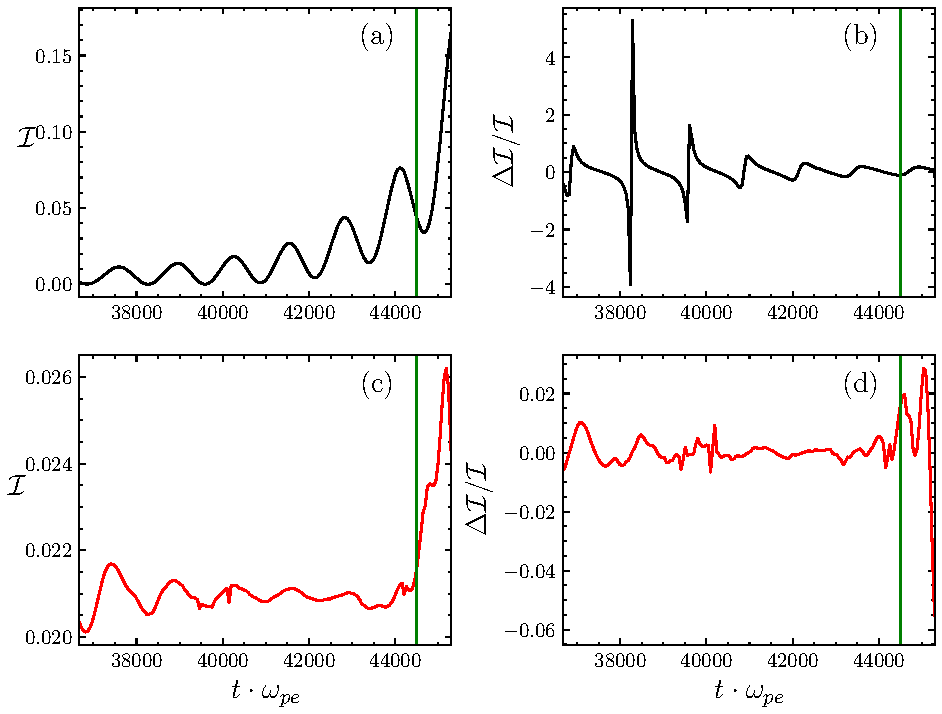
\includegraphics[scale=0.5]{img/adiaI.pdf}
    \caption{Time variation and  relative change of $\mathcal{I}$ for the test particle in the static (the black lines) and  real-time resonance  frames (the red lines). The green vertical line denotes the critical time when the conservation of $\mathcal{I}$ is violated.
    }
    \label{fig.I}
\end{figure}
To quantitatively show the adiabaticity, we numerically calculate the area of the phase loop and show its time variation 
and the relative error of the adiabatic invariant $\mathcal{I}(t)$ in Fig. \ref{fig.I}.
Unlike the static frame, the variation of $\mathcal{I}$ is less than $2\%$ in the reference frame following with the resonance, as seen in Fig. \ref{fig.I}(d). 
The adiabatic invariant $\mathcal{I}$ and the validity of the adiabaticity are shown to be conserved. 
The variation becomes large until the particle approaches the equator, where the wave amplitude is small, and the particle can be released from the wave potential well. 
The releasing of trapped particle, which is reported in the particle in cell (PIC) simulation \cite{tao_trap-release-amplify_2021}, could be a potential reason for the violation of the adiabatic motion.


The nonlinear energetic particle current $j_p$ is obtained from the velocity integral of the perturbed distribution function 
\cite{zheng2024}
\begin{equation}\label{eq.ep_current}
    \begin{aligned}
j_p(s,t) & = -\frac{1}{ 4 \pi } n_h k \iiint \sqrt{2 \omega_{ce}(s)(\mathcal{J}+\Omega+\Pi)} 
 \\
 &\times f(\xi,\Omega,\mathcal{J};s(t),t)e^{\imath \xi} \rm d \xi \rm d \Omega \rm d \mathcal{J}~.
    \end{aligned}
\end{equation}
where $n_h$ is the density of the energetic particle.
With the adiabatic approximation, we can greatly reduce the description of the trapped particle distribution and the energetic particle current.
Since the equilibrium distribution does not contribute to the current, the nonlinear current is directly determined by 
the deviation from the unperturbed distribution, i.e., the depth of the hole,
$\Delta f$.
The depth of the hole can be written as the function of the adiabatic invariant, i.e., $\Delta f(s,\mathcal{J},\mathcal{I},\xi,t)$.
Replacing $f$ by $\Delta f$, and directly change the differential element $\mathrm{d}\xi\mathrm{d}\Omega$ is changed to $\mathrm{d}\mathcal{I}\mathrm{d}\psi$, where $\psi$ is the angle variable of $\mathcal{I}$, then the current integral  Eq.~(\ref{eq.ep_current}) becomes 
%and write  the integral as
% \begin{equation}
% \begin{aligned}
%     j_p(s,t) & \approx - \frac{n_h k}{4\pi} \int\mathrm{d} \mathcal{J} \sqrt{2 \omega_{ce} (\mathcal{J} + \Pi(t))}
%     \\
%     &\times \int_0^{\mathcal{I}_{\mathrm{s p x}}}  \mathrm{d}\mathcal{I}  \oint \mathrm{d}\psi  \Delta f(s,\mathcal{J},\mathcal{I},\xi,t)e^{\imath \xi}  ~.
% \end{aligned}
% \end{equation}
% The differential area element $\mathrm{d}\xi\mathrm{d}\Omega$ is changed to $\mathrm{d}\mathcal{I}\mathrm{d}\psi$, where $\psi$ is the angle variable of $\mathcal{I}$.
% From the Jacobi of the differential element, the integral over $\psi$ is
% \begin{equation}
%     \begin{aligned}
%       \oint f \mathrm{d}\psi & = \oint f \frac{\mathrm{d}\Omega}{\mathrm{d}\mathcal{I}}\mathrm{d}\xi = \frac{\partial H}{\partial \mathcal{I}} \oint f \frac{\mathrm{d}\Omega}{\mathrm{d} H}\mathrm{d}\xi = \dot{\psi}\oint \frac{f}{\Omega} \mathrm{d}\xi
%       \\
%       &\equiv 2 \pi \langle f \rangle,
%     \end{aligned}
% \end{equation}
%Thus the current integral becomes
\begin{equation}\label{eq.adiabatic_current}
\begin{aligned}
    j_p(s,t)  &\approx -  \frac{n_h k}{2} \int\mathrm{d} \mathcal{J}  \sqrt{2\omega_{ce} (\mathcal{J} + \Pi)} \\
    & \times 
    \int_0^{\mathcal{I}_{\mathrm{s p x}}}\mathrm{d}\mathcal{I}  \langle \Delta f(s,\mathcal{J},\mathcal{I},\xi,t)e^{\imath \xi} \rangle  ~.
\end{aligned}
\end{equation}
where 
the $\Omega$ in the square root has been  neglected since $\Omega \simeq 0$
and 
%$\langle\cdots\rangle$ 
from the Jacobi of the differential element, the integral over $\psi$ can be represented as the bounce average defined as 
\cite{berk1999}
\begin{equation}
    \begin{aligned}
       \frac{1}{2\pi}\oint f d\psi = & \oint \frac{ f }{\Omega}\mathrm{d}\xi \bigg/ \oint \frac{1}{\Omega} \mathrm{d} \xi   \equiv\langle f \rangle 
%      \oint f \mathrm{d}\psi & = \oint f \frac{\mathrm{d}\Omega}{\mathrm{d}\mathcal{I}}\mathrm{d}\xi = 
%\frac{\partial H}{\partial \mathcal{I}} \oint f \frac{\mathrm{d}\Omega}{\mathrm{d} H}\mathrm{d}\xi 
%= \dot{\psi}\oint \frac{f}{\Omega} \mathrm{d}\xi
      \\
    \end{aligned}
\end{equation}
% following the definition in Ref. 
Note that $\Delta f$ can be expanded in powers of  a small parameter describing the change of parameters during the bounce motion and then the bounce averages in Eq.~(\ref{eq.adiabatic_current}) become 
 \cite{berk1999} 
\begin{equation}
    \begin{aligned}
    \langle\Delta f \sin \xi \rangle &\simeq \alpha \Delta f_0 ~, \\ 
    \langle \Delta f \cos \xi \rangle &\simeq  \Delta f_0 \langle \cos \xi \rangle ~.
    \end{aligned}
\end{equation}
We further assume that $\Delta f_0$ is independent of $\mathcal{I}$, which implies that the depth of the hole is flat within the enclosed hole area, i.e., the water bag approximation \cite{omura_theory_2008,hezaveh2021}. 
Therefore, the integral over $\mathcal{I}$ only depend on the $\mathcal{I}_\mathrm{spx}$ which is the 
 adiabatic invariant on the separatrix. 
According to Eq. (\ref{eq.def_I}), we have
\begin{equation}
    \int^{\mathcal{I}_\mathrm{s p x}}_0 \mathrm{d}\mathcal{I} = \mathcal{I}_\mathrm{s p x} \equiv {\frac{1}{2\pi}} \oint_\mathrm{s p x} \Omega (\xi) \mathrm{d} \xi~,
\end{equation}
where the boundary of the trapped particle phase space hole can be analytically given as
\begin{equation}\label{eq.bound}
    \Omega(\xi) = \pm \frac{\omega_b}{k^2} \sqrt{2 (e_\mathrm{spx}-\cos \xi - \alpha \xi)}~,
\end{equation}
and $e_\mathrm{spx}= \cos\xi_1 - \alpha \xi_1 = \cos\xi_2 - \alpha \xi_2$, where $\xi_1$ and $\xi_2$ indicate the two boundaries of the trapping region at $\Omega = 0$ \cite{omura2008}.
%and $e_\mathrm{spx}= \cos\xi_X - \alpha \xi_X = \cos\xi_C - \alpha \xi_C$, where $\xi_X$ denotes the location of the saddle point of the hole (X point), and $\xi_C$ denotes the other boundary of the trapping region at $\Omega = 0$ (C point) \cite{omura2008}.
Then the current integral becomes  
\begin{equation}\label{eq.adi_J}
    \begin{aligned}
    j_p(s,t) & \approx \frac{n_h }{4\pi} \frac{\sqrt{2} \omega_b}{k}  \left(m_\mathrm{s p x}+\imath ~ n_\mathrm{s p x}\right) \\
    & \times  \int \mathrm{d} \mathcal{J} \sqrt{ \omega_{c e}(\mathcal{J}+\Pi)} \Delta f_0(\mathcal{J},s,t) ~,
    \end{aligned}
\end{equation}
where
\begin{equation}\label{eq.function}
    \begin{aligned}
        m_\mathrm{spx}(\alpha) & = \langle  \cos \xi \rangle\oint_\mathrm{s p x} \mathrm{d} \xi \sqrt{e_\mathrm{s p x}-\cos \xi-\alpha \xi}
        \\
        & =\oint_\mathrm{s p x} \mathrm{d} \xi \cos \xi \sqrt{e_\mathrm{s p x}-\cos \xi-\alpha \xi}
        \\
        n_\mathrm{spx}(\alpha) &  = \alpha \oint_\mathrm{s p x} \mathrm{d} \xi \sqrt{e_\mathrm{s p x}-\cos \xi-\alpha \xi}.
    \end{aligned}
\end{equation}
\begin{figure}
    \centering
    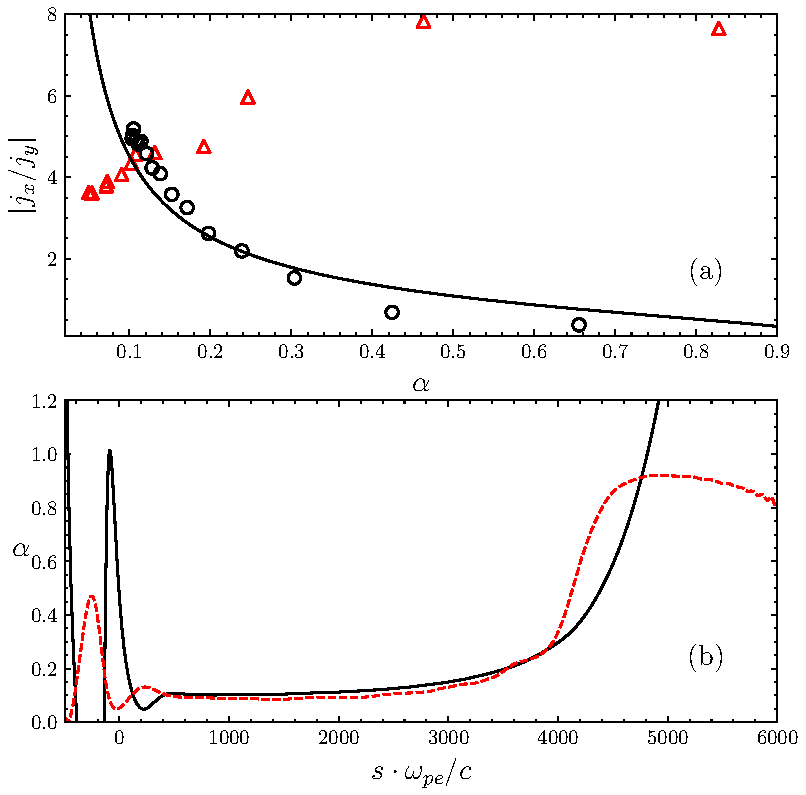
\includegraphics[scale=0.5]{img/alpha.pdf}
    \caption{(a) Current ratio versus the inhomogeneous parameter $\alpha$. The scattered points are obtained at difference spatial locations from the simulation, the triangles are obtained from near the equator region while circus are obtained from the downstream region. 
    The solid curve is the results from adiabatic approximation Eq. (\ref{eq.adia_relation}). 
    (b) Spatial distribution   of the parameter $\alpha$ at $t\simeq41564\omega_{pe}^{-1}$ obtained  from the definition  Eq. (\ref{eq.alpnew}) (red dashed line) and  from adiabatic relation Eq. (\ref{eq.adia_relation}) (black solid line).
    }
    \label{fig.adiabatic}
\end{figure}

The temporospatial evolution of the nonlinear current only depends on the integral over the slowly varying scale $\mathcal{J}$ and the parameter $\alpha$ defined in Eq. (\ref{eq.alpnew}). 
The $\mathcal{J}$ integral can be calculated further with the adiabatic motion of the trapped particle along the magnetic field line \cite{summers2012}, while the integrals $m_\mathrm{spx}$ and $n_\mathrm{spx}$ can be numerical integrated from Eq. (\ref{eq.function}).
Since the Vlasov simulation is performed with Hamiltonian Eq.~(\ref{eq.H_lab})
\cite{zheng2023b,zheng2024}, the phase of the current $j_p$ in the Vlasov simulation also differs $\delta \phi$ with the current relation in Eq. (\ref{eq.adi_J}).
To compare and verify the adiabatic theory, we should also take into account this additional phase, i.e., $j^\prime_{p} = j_p \cdot e^{-\imath \delta \phi}$, where $j_p$ is the current from the Vlasov simulation. 
From Eqs.~(\ref{eq.adi_J}) and (\ref{eq.function}), we can find that the ratio of the real to imaginary components of $j^\prime_{p}=j_x+\imath~ j_y$ is a function of the inhomogeneous parameter, 
\begin{equation}\label{eq.adia_relation}
\frac{j_x}{j_y} 
= \frac{{\Re}(j^\prime_p)}{{\Im}(j^\prime_p)} 
= \frac{m_\mathrm{spx}(\alpha)}{n_\mathrm{spx}(\alpha)}
\end{equation}

By numerically solve the integral in Eq. (\ref{eq.function}), we obtain an explicit relation of the current ratio with respect to $\alpha$, as shown in Fig. \ref{fig.adiabatic}(a). 
To verify the validity of the relation, we select various spatial locations at $t\simeq41564\omega_{pe}^{-1}$ from the Vlasov simulation \cite{zheng2023b,zheng2024} and calculate the $\alpha$ from the definition Eq. (\ref{eq.alpnew}) and the corresponding current ratio.
It is shown that the values obtained in the Vlasov simulation  well agree with the adiabatic predictions in the propagation region of chorus waves (black circles).
The  relation  Eq. (\ref{eq.adia_relation}) can also be applied as an alternative way for evaluating the inhomogeneous parameter $\alpha$ from the energetic particle current.
This provides a new way to obtain the inhomogeneous parameter $\alpha$ which is important to study the wave-particle interaction and the chirping behavior \cite{tao_theoretical_2020,omura2008}.
Near the equator region where the chorus is triggered (red triangles), the adiabatic approximation is no longer valid.

The adiabaticity is also examined from the spatial distribution of $\alpha$ in Fig. \ref{fig.adiabatic}(b), where we compare the value calculated from the definition Eq. (\ref{eq.alpnew}) and the adiabatic current relation Eq. (\ref{eq.adia_relation}). 
In the source region near the equator $s=0$, the $\alpha$  quickly rises to large values and there exists a clear discrepancy between the values of $\alpha$ from the definition and adiabatic relation, indicating  the violation of the adiabatic approximation.
In the broad region of the wave propagation $s>0$,  the $\alpha$ values  from the two methods show good agreement,  which means that the adiabatic approximation is effective.
In the far region over $s\simeq4000c/\omega_{pe}$ where the  $\alpha$  goes to high values, the adiabaticity is also invalid, simply because the holes have not formed yet near the far outer boundary. 
